\chapter{Concept Learning (Machine Learning)}
\label{s:conceptLearning}
\chapterquote{Een hypothese vormt een stimulans om naar bepaalde eigenschappen te zoeken of ze juist te verwaarlozen, of zelfs te ontkennen.}{Umberto Eco, Italiaans schrijver en criticus (1932-)}
\termen{Machine learning} is een probleem waarbij we proberen een machine in staat te stellen zelf te leren vanuit ervaring. In deze cursus gaan we alleen dieper in op \termen{Concept Learning}. Hierbij proberen we de machine een concept te laten leren. Dit moet vervolgens resulteren in een algoritme die het beslissingsprobleem kan oplossen: ``behoort een bepaalde situatie tot het gekende concept?''. Met andere woorden we geven een bepaalde situatie $s$ en we verwachten dat de machine kan antwoorden met juist of fout of de situatie die we tonen wel degelijk tot het concept behoort. Om de machine te trainen in het begrijpen van het concept geven we een hoeveelheid testdata: een reeks situaties waarbij we zelf vermelden of de situatie deel uitmaakt van het beoogde concept. Algemeen kunnen we dus stellen dat het algoritme in staat moet zijn om de verzameling van situaties op te splitsen in juiste of foute. Dit proces is uiteraard niet deterministisch, we hebben immers alleen maar de volledige notie van het concept indien we de volledige verzameling situaties als testdata zouden ingeven, in dat geval is het algoritme uiteraard zinloos.
\paragraph{}
Formeel kunnen we ieder probleem waarbij we de machine het concept willen laten leren als volgt voorstellen:
\begin{itemize}
 \item Een set van ``\termen{events}'' $\Ee$ dit zijn de parameters waarover we informatie hebben in ons probleem. Bijvoorbeeld ``First Name'', ``Country'' en ``Job''.
 \item Een ongekende doelfunctie $c$, deze functie beslist iedere situatie in het probleem. $c:\Ee\rightarrow\Bb=\left\{\true,\false\right\}$
 \item Een set testdata $D$: situaties waarvoor $c$ wel gekend is
 \item Een hypothesetaal die kan uitdrukken welke situaties wel en welke niet tot het concept behoren.
\end{itemize}
We zijn op zoek naar een hypothese $h$ zodat geldt voor alle testdata $D$:
\begin{equation}
\forall d\in D:d\mbox{ is waar volgens } h\leftrightarrow c\left(d\right)
\end{equation}
\paragraph{}
Voor dit probleem zijn in de loop der tijd verschillende oplossingen bedacht zoals neurale netwerken. De oplossing die we hier behandelen heet \termen{Version Spaces}.
\section{Leidend Voorbeeld: Solliciteren}
\begin{leftbar}
Een bedrijf wil enkele nieuwe werknemers aanwerven. Er reageren echter een groot aantal mensen op de vacature. Manueel selecteren van de sollicitanten die een gesprek krijgen lijkt dan ook onbegonnen werk. We zullen in dit hoofdstuk een manier uitwerken zodat een programma op basis van enkele beslissingen die door de personeelsdirecteur zijn gemaakt, de rest van de sollicitanten zal indelen. Er worden slechts enkele parameters uit het curriculum vitae gebruikt: de studie, de leeftijd (dit is overigens verboden) en de hobby van de persoon in kwestie. Bovendien zullen we in dit voorbeeld slechts enkele waarden invullen. We ordenen en groeperen de verschillende mogelijke waarden volgens figuur \ref{fig:sollicitatieConceptTree}. De testdata wordt weergegeven in tabel \ref{tbl:sollicitatieTestData}.
\end{leftbar}
\begin{figure}[htb]
\centering
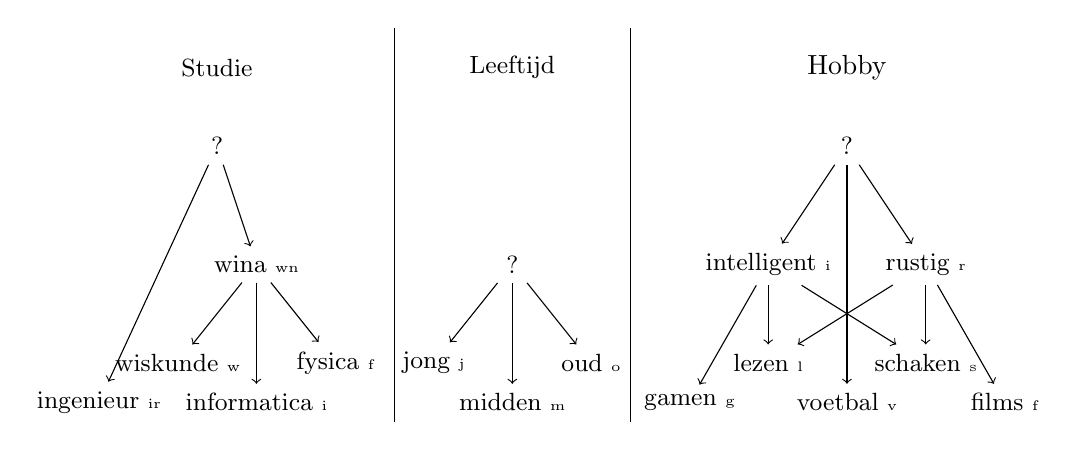
\begin{tikzpicture}
\node (s) at (-3.75,0) {\small Studie};
\node (sG) at (-3.75,-1) {\small ?};
\node (si) at (-5.25,-4.25) {\small ingenieur \tiny ir};
\draw[->] (sG) -- (si);
\node (sw) at (-3.25,-2.5) {\small wina \tiny wn};
\draw[->] (sG) -- (sw);
\node (swf) at (-4.25,-3.75) {\small wiskunde \tiny w};
\draw[->] (sw) -- (swf);
\node (swi) at (-3.25,-4.25) {\small informatica \tiny i};
\draw[->] (sw) -- (swi);
\node (sww) at (-2.25,-3.75) {\small fysica \tiny f};
\draw[->] (sw) -- (sww);
\draw (-1.5,0.5) -- (-1.5,-4.5);
\node (a) at (0,0) {\small Leeftijd};
\node (aG) at (0,-2.5) {\small ?};
\node (ay) at (-1,-3.75) {\small jong \tiny j};
\draw[->] (aG) -- (ay);
\node (am) at (0,-4.25) {\small midden \tiny m};
\draw[->] (aG) -- (am);
\node (ao) at (1,-3.75) {\small oud \tiny o};
\draw[->] (aG) -- (ao);
\draw (1.5,0.5) -- (1.5,-4.5);
\node (h) at (4.25,0) {Hobby};
\node (hG) at (4.25,-1) {\small ?};
\node (hi) at (3.25,-2.5) {\small intelligent \tiny i};
\draw[->] (hG) -- (hi);
\node (hig) at (2.25,-4.25) {\small gamen \tiny g};
\draw[->] (hi) -- (hig);
\node (hil) at (3.25,-3.75) {\small lezen \tiny l};
\draw[->] (hi) -- (hil);
\node (hv) at (4.25,-4.25) {\small voetbal \tiny v};
\draw[->] (hG) -- (hv);
\node (hr) at (5.25,-2.5) {\small rustig \tiny r};
\draw[->] (hG) -- (hr);
\draw[->] (hr) -- (hil);
\node (hrs) at (5.25,-3.75) {\small schaken \tiny s};
\draw[->] (hi) -- (hrs);
\draw[->] (hr) -- (hrs);
\node (hrf) at (6.25,-4.25) {\small films \tiny f};
\draw[->] (hr) -- (hrf);
\end{tikzpicture}
\caption{Conceptboom van de sollicitatie}
\label{fig:sollicitatieConceptTree}
\end{figure}
\begin{table}[htb]
\centering
\begin{tabular}{c|l|l|l|c}
\#&Studie&Leeftijd&Hobby&+/--\\\hline
1&fysica&midden&voetbal&--\\
2&informatica&jong&schaken&+\\
3&ingenieur&oud&gamen&--\\
4&wiskunde&jong&lezen&+\\
5&fysica&jong&gamen&+\\
6&ingenieur&jong&gamen&--
\end{tabular}
\caption{Testdata van het sollicitatie voorbeeld}
\label{tbl:sollicitatieTestData}
\end{table}
% \section{Leidend Voorbeeld: Muziek}
% \label{ss:versionSpacesExample}
% \begin{leftbar}
% Het leidend voorbeeld komt dit keer uit de muziek. We gaan uit van een fragment uit een muziekstuk. We willen een machine het concept achter het muziekstuk laten leren. Hierdoor moet de machine op termijn in staat zijn om voor een ander fragment te determineren of het al dan niet tot hetzelfde muziekstuk hoort. We willen reeds vooraf melden dat de concrete parameters die we in dit voorbeeld gebruiken niet voldoen om dit te determineren. Dit voorbeeld is dan ook louter een illustratie.
% \paragraph{Notenleer}
% We zullen het concept leren aan de hand van de noten die in het stuk gespeeld worden. We beschouwen bovendien slechts twee karakteristieken: toonhoogte en lengte. Op een partituur bepaald de vorm van de noot de lengte van de noot. Zoals weergegeven op figuur \ref{fig:notesLength}. Verder bepaald de hoogte van de noot op de notenbalk de toonhoogte. We beschouwen slechts een deel van de beschikbare toonhoogtes.
% \end{leftbar}
% \begin{figure}[htb]
% \centering
% \caption{Verschillende lengtes van de noten}
% \label{fig:notesLength}
% \end{figure}
% \begin{figure}
% \begin{tikzpicture}
% \node (S1) at (0,0) {?};
% \end{tikzpicture}
% \caption{Conceptboom van muziek.}
% \label{afb:muziekConceptTree}
% \end{figure}
% Als leidend voorbeeld willen we een machine een voor ons zelf onbekend concept concept in het kaarstpel ``Manillen'' laten leren. Hiervoor zullen we tabel \ref{tbl:manillenConceptTest} als test-data invoeren. Verder zullen we de eigenschapshi\"erarchie van afbeelding \ref{fig:manillenConceptHierarchy} gebruiken.
% \begin{table}[htb]
% \centering
% \begin{tabular}{|c|c|c|}
% \hline
% Waarde&Kleur&Resultaat\\
% \hline
% \hline
% 7&$\diamondsuit$&+\\\hline
% A&$\clubsuit$&-\\\hline
% Q&$\heartsuit$&-\\\hline
% 9&$\heartsuit$&+\\\hline
% 8&$\clubsuit$&-\\\hline
% \end{tabular}
% \caption{Test-data voor ``Manillen''}
% \label{tbl:manillenConceptTest}
% \end{table}
% \begin{figure}[htb]
% \centering
% \begin{tikzpicture}
% \def\dxx{1.5};
% \def\dxy{0.75};
% \def\dxz{6};
% \def\dxa{2.5};
% \def\dxb{0.75};
% \def\dy{-1};
% \node (Waarde) at (0,0) {?};
% \node (A) at (-\dxa,\dy) {A};
% \draw (Waarde) -- (A);
% \node (Numbers) at (0,\dy) {Numbers};
% \draw (Waarde) -- (Numbers);
% \node (Pictures) at (\dxa,\dy) {Pictures};
% \draw (Waarde) -- (Pictures);
% \node (7) at (-1.5*\dxb,2*\dy) {7};
% \draw (Numbers) -- (7);
% \node (8) at (-0.5*\dxb,2*\dy) {8};
% \draw (Numbers) -- (8);
% \node (9) at (0.5*\dxb,2*\dy) {9};
% \draw (Numbers) -- (9);
% \node (10) at (1.5*\dxb,2*\dy) {10};
% \draw (Numbers) -- (10);
% \node (J) at (\dxa-\dxb,2*\dy) {J};
% \draw (Pictures) -- (J);
% \node (Q) at (\dxa,2*\dy) {Q};
% \draw (Pictures) -- (Q);
% \node (K) at (\dxa+\dxb,2*\dy) {K};
% \draw (Pictures) -- (K);
% \node (Kleur) at (\dxz,0) {?};
% \node (Red) at (\dxz-0.5*\dxx,\dy) {Red};
% \draw (Kleur) -- (Red);
% \node (Black) at (\dxz+0.5*\dxx,\dy) {Black};
% \draw (Kleur) -- (Black);
% \node (H) at (\dxz-0.5*\dxx-0.5*\dxy,2*\dy) {$\heartsuit$};
% \draw (Red) -- (H);
% \node (D) at (\dxz-0.5*\dxx+0.5*\dxy,2*\dy) {$\diamondsuit$};
% \draw (Red) -- (D);
% \node (S) at (\dxz+0.5*\dxx-0.5*\dxy,2*\dy) {$\spadesuit$};
% \draw (Black) -- (S);
% \node (C) at (\dxz+0.5*\dxx+0.5*\dxy,2*\dy) {$\clubsuit$};
% \draw (Black) -- (C);
% \end{tikzpicture}
% \caption{Eigenschapshi\"erarchie van ``Manillen''}
% \label{fig:manillenConceptHierarchy}
% \end{figure}
\section{Version Spaces}
Version spaces is een symbolische oplossingsmethode, waarbij aan de hand van een \termen{hypothesetaal} een concept geleerd wordt, die vervolgens de overige data kan beoordelen.
\subsection{Na\"ieve benadering}
\label{sss:versionSpacesNaif}
Een eerste en zeer na\"ieve oplossingsmethode is ervan uitgaan dat alleen de situaties die we gezien hebben in de testdata die positief zijn, ook de situaties zijn die tot het concept behoren. In dat geval bouwen we niets anders dan een zoekalgoritme die kijkt of de ingegeven situatie bij de testdata positief vermeld stond en dan juist teruggeeft, indien niet geeft het vals terug. Een even slechte keuze is natuurlijk net het omgekeerde: alle situatie voldoen aan het concept tenzij de testdata dit tegenspreekt. Aan deze oplossingen hebben we natuurlijk helemaal niets: het is de bedoeling dat we iets kunnen zeggen over situaties die we nog niet kennen. Bij het eerste geval moet we immers het concept \termen{veralgemenen} (verbreden), in het tweede voorbeeld moet we het concept kunnen \termen{specificeren} (vernauwen).
\begin{leftbar}
Concreet betekent dit dus dat we bij het voorbeeld alleen juist teruggeven op (informatica, jong, schaken), (wiskunde, jong, lezen) en (fysica, jong, gamen). In het tweede geval is het resultaat altijd juist, behalve indien er (fysica, midden, voetbal), (ingenieur, oud, gamen) en (ingenieur, jong, gamen) ingevoerd wordt. 
\end{leftbar}
\subsection{Oplossing: bouwen van een hypothesetaal}
De oplossing van dit probleem bestaat eruit een taal te ontwikkelen, die een concept kan uitleggen: de hypothesetaal. Deze taal moet het mogelijk maken een verzameling van hypotheses of beschrijvingen te genereren: de \termen{hypotheseruimte}. Vervolgens kan een concept alleen uitgelegd worden aan de hand van \'e\'en van de elementen uit de hypotheseruimte. Een goede hypothesetaal moet het probleem van zinloze beschrijvingen tegengaan, zoals gesteld in \ref{sss:versionSpacesNaif}. Daarnaast moet het de machine tot veralgemening of specifi\"ering dwingen, die in de meeste gevallen nuttig is (zo is bijvoorbeeld een veralgemening naar een concept ``alles is toegelaten'', meestal geen goed idee).
\paragraph{}
In deze cursussen ontwikkelen we een hypothesetaal die gezien kan worden als een conjunctie van gelijkheden. Hierbij zien we een hypothese als een rij waarbij ieder element een bepaalde eigenschap is van de situatie die we kunnen meten.
\begin{leftbar}
Concreet kunnen volgende voorbeelden, hypotheses zijn voor het leidend voorbeeld met als parameters $\left[\mbox{Studie}, \mbox{Leeftijd}, \mbox{Hobby}\right]$ zijn:
\begin{itemize}
 \item $\left[\mbox{wiskunde},\mbox{jong},\mbox{lezen}\right]$: Alle jonge wiskundigen die als hobby lezen
 \item $\left[\mbox{informatica},\mbox{?},\mbox{?}\right]$: Alle informatici
 \item $\left[\mbox{wina},\mbox{?},\mbox{?}\right]$: Alle mensen die wiskunde informatica of fysica gestudeerd hebben (de twee vorige hypotheses behoren hier dus ook toe)
 \item $\left[\mbox{ingenieur},\mbox{oud},\mbox{?}\right]$: Alle oude ingenieurs
 \item $\left[\mbox{?},\mbox{jong},\mbox{rustig}\right]$: Alle jonge mensen die een rustige hobby uitoefenen
 \item $\left[\mbox{?},\mbox{?},\mbox{?}\right]$: Iedereen
 \item $\perp$: Niemand
\end{itemize}
\end{leftbar}
Hierbij beperken we de concepten dus niet noodzakelijk tot een equivalentie van alle waarden. Het vraagteken (?) betekent dat deze parameter niet relevant is voor het concept, in dat geval betekent dit dat wat er ook staat op deze plaats in de situatie, dit niet zal bepalen of we de situatie verwerpen. Anderzijds kunnen we ook een hi\"erarchie opbouwen in waarden die bij de parameters horen. Zo staat ``rustig'' duidelijk boven ``lezen'' en ``schaken'', en staat ``wina'' boven ``fysica'' en ``wiskunde'' (zie ook de hi\"erarchie van het leidend voorbeeld op figuur \ref{fig:sollicitatieConceptTree}). Tot slot bestaat er ook nog een lege hypothese: $\perp$, in dat geval zal iedere situatie niet tot het concept behoren. Het spreekt voor zich dat $\left[\mbox{?},\mbox{?},\mbox{?}\right]$ en $\perp$ niet echt de beoogde oplossingen zijn. Daar we hierbij eenvoudigweg stellen dat respectievelijk alles en niets tot het concept behoren.
\subsection{De Inductieve Leer-hypothese}
Zal deze taal wel volstaan om een bepaald concept te leren? Hierbij beroepen we ons op de Inductieve Leer-hypothese, dat is een theorema dat stelt:
\begin{theorem}
Indien we een hypothese $h$ vinden die de doelfunctie $c$ op de testdata $D$ voldoende benadert, dan zal $h$ $c$ ook voldoende benaderen op situaties die niet behoren tot $D$.
\end{theorem}
Met dit theorema zijn we in staat een minder na\"ief algoritme, \termen{Find-S}, te bouwen die een concept leert door middel van generalisatie. Dit algoritme vertrekt van een $\perp$ hypothese, met andere woorden het verwerpt iedere situatie die het tegenkomt. Wanneer we de testdata evalueren zal het bij een positieve test-situatie de hypothese minimaal generaliseren. Dit resulteert in een hypothese die altijd waar is bij positieve situaties in de testdata. Dit is echter onvoldoende omdat negatieve test-situaties niet altijd als fout beoordeeld zullen worden (we kunnen dus stellen dat de hypothese de testdata niet voldoende benadert). Toch zal dit algoritme \'e\'en van de elementen vormen in de oplossing. Dit algoritme wordt beschreven in \algref{alg:findS}.
\begin{algorithm}[htb]                      % enter the algorithm environment
\caption{Find-S}          % give the algorithm a caption
\label{alg:findS}                           % and a label for \ref{} commands later in the document
\begin{algorithmic}[1]                    % enter the algorithmic environment
\STATE $h\leftarrow\perp$
\FORALL{$d\in D\wedge c\left(d\right)$}
\IF{$\neg\hypothesiscovers{h,d}$}
\STATE $h\leftarrow\minimalgeneralisationthatcovers{h,d}$
\ENDIF
\ENDFOR
\end{algorithmic}
\end{algorithm}
Uiteraard is het kiezen van de minst veralgemenende hypothese niet deterministisch bepaald. Algemeen zijn er echter een aantal richtlijnen:
\begin{itemize}
 \item Events die voldoende algemeen waren om de situatie toch te doen slagen worden niet aangepast
 \item Events die in de hypothese niet voldoende algemeen waren worden veralgemeend door een ouder-waarde te kiezen die zowel de oorspronkelijke waarde bevat en de waarde van de falende situatie
\end{itemize}
Concreet betekent dit dus dat bij de eerste veralgemening eenvoudigweg de situatie als nieuwe hypothese gezien wordt. Verder zijn er soms verschillende ouder-waarden die de twee waarden ondersteunen. In dat geval dient er eenvoudigweg \'e\'en van de mogelijkheden gekozen te worden.
\paragraph{}
Find-S is hierdoor niet geschikt om tot een goede hypothese te komen, zowel het niet-deterministisch karakter als het afleveren van foute hypotheses maken het ongeschikt. Verder is het algoritme niet in staat inconsistenties in de data te detecteren, wanneer eenzelfde situatie eerst positief en daarna negatief voorkomt. Voordelen van Find-S zijn dan weer dat het zowel een goede tijds- \bigoh{n} als geheugencomplexiteit \bigoh{1} bevat.
\begin{leftbar}
Indien we Find-S toepassen op het leidend voorbeeld, kan dit tot een scenario leiden zoals bij tabel \ref{tbl:solliciterenFindS}. Merk op dat de keuze van generalisatie bij sample 4 niet deterministisch bepaald is. We kunnen dus afhankelijk van de details van de implementatie van Find-S tot een andere hypothese komen.
\end{leftbar}
\begin{table}[htb]
\centering
\begin{tabular}{c|c|c}
\#&Hypothese&Alternatieven\\
\hline
I&$\perp$\\
2&$\left[\mbox{informatica},\mbox{jong},\mbox{schaken}\right]$&\\
4&$\left[\mbox{wina},\mbox{jong},\mbox{rustig}\right]$&$\left[\mbox{wina},\mbox{jong},\mbox{intelligent}\right]$\\
5&$\left[\mbox{wina},\mbox{jong},\mbox{?}\right]$&
\end{tabular}
\caption{Find-S toegepast op het leidend voorbeeld.}
\label{tbl:solliciterenFindS}
\end{table}
\paragraph{}
De tegenhanger van Find-S is \termen{Dual Find-S} hierbij wordt uitgegaan van het meest algemene geval ($\left[\mbox{?},\mbox{?},\ldots,\mbox{?}\right]$), vervolgens wordt bij iedere negatieve test-situatie die niet aan de hypothese voldoet de hypothese minimaal gespecificeerd. Zoals beschreven in \algref{alg:dualFindS}.
\begin{algorithm}[htb]                      % enter the algorithm environment
\caption{Dual Find-S}          % give the algorithm a caption
\label{alg:dualFindS}                           % and a label for \ref{} commands later in the document
\begin{algorithmic}[1]                    % enter the algorithmic environment
\STATE $h\leftarrow\left[\mbox{?},\mbox{?},\ldots,\mbox{?}\right]$
\FORALL{$d\in D\wedge\neg c\left(d\right)$}
\IF{$\hypothesiscovers{h,d}$}
\STATE $h\leftarrow\minimalspecialisationthatnotcovers{h,d}$
\ENDIF
\ENDFOR
\end{algorithmic}
\end{algorithm}
Opnieuw gelden hier dezelfde opmerkingen als bij Find-S.
\begin{leftbar}
We passen opnieuw het leidend voorbeeld toe, op Dual Find-S. Het resultaat hiervan wordt weergegeven in tabel \ref{tbl:sollicitatieDualFindS}. Opnieuw stellen we vast dat we tussen verschillende opties kunnen kiezen. Bovendien kan de uiteindelijke hypothese onmogelijk voldoen. Indien we de positieve voorbeelden hierop testen falen deze allemaal!
\end{leftbar}
\begin{table}[htb]
\centering
\begin{tabular}{c|c|c}
\#&Hypothese&Alternatieven\\
\hline
I&$\left[?,?,?\right]$&\\
1&$\left[?,?,\mbox{intelligent}\right]$&$\left[\mbox{ir},?,?\right],\left[\mbox{w},?,?\right],\left[\mbox{i},?,?\right],\left[?,\mbox{j},?\right],\left[?,\mbox{o},?\right],\left[?,?,\mbox{r}\right]$\\%\left[\mbox{},\mbox{},\mbox{}\right]
3&$\left[?,\mbox{midden},\mbox{intelligent}\right]$&$\left[\mbox{wina},?,?\right],\left[?,?,\mbox{lezen}\right],\left[?,?,\mbox{schaken}\right]$\\
6&$\left[?,\mbox{midden},\mbox{intelligent}\right]$&(vorige hypothese voldoet)
\end{tabular}
\caption{Dual Find-S toegepast op het leidend voorbeeld.}
\label{tbl:sollicitatieDualFindS}
\end{table}
\subsection{Version Spaces: het idee}
Het idee van Version Spaces is nochtans gebaseerd op Find-S en Dual Find-S. Maar de twee algoritmen worden tegelijk uitgevoerd, en bovendien worden alle nieuwe minimale generalisaties en specificaties bijgehouden in een boomstructuur in tegenstelling tot het kiezen van eentje bij Find-S en Dual Find-S. Nadien worden alle mogelijke generalisaties afgewogen tegen alle mogelijke specificaties. We zullen het algoritme hiervoor stap voor stap opbouwen en verschillende optimalisaties implementeren. Hiervoor beginnen we met een grofstructuur van hoe het algoritme er dient uit te zien in \algref{alg:versionSpacesBase}.
\begin{algorithm}[htb]                      % enter the algorithm environment
\caption{Grofstructuur van het Version-Spaces algoritme}          % give the algorithm a caption
\label{alg:versionSpacesBase}                           % and a label for \ref{} commands later in the document
\begin{algorithmic}[1]                    % enter the algorithmic environment
\STATE\COMMENT{Verzameling van hypotheses die vanuit de meest algemene hypothese vertrekken}
\STATE $G\leftarrow\left\{\left[\mbox{?},\mbox{?},\ldots,\mbox{?}\right]\right\}$
\STATE\COMMENT{Verzameling van hypotheses die vanuit de meest specifieke hypothese vertrekken}
\STATE $S\leftarrow\left\{\perp\right\}$
\FORALL{$d\in D$}
\IF{$\neg\notempty{G}\vee\neg\notempty{S}$}
\STATE\COMMENT{Dit treed op indien de testdata tegenstrijdige informatie bevat}
\RETURN $\failure$
\ENDIF
\IF{$c\left(d\right)$}
\STATE\COMMENT{positieve test-situatie}
\FORALL{$h\in S$}
\IF{$\neg\hypothesiscovers{h,d}$}
\STATE\COMMENT{Een hypothese heeft een probleem met de test-situatie}
\STATE\COMMENT{Oplossing}
\STATE $\ldots$
\ENDIF
\ENDFOR
\STATE\COMMENT{Alle problemen zijn opgelost}
\ELSE
\STATE\COMMENT{negatieve test-situatie}
\FORALL{$h\in G$}
\IF{$\hypothesiscovers{h,d}$}
\STATE\COMMENT{Een hypothese heeft een probleem met de test-situatie}
\STATE\COMMENT{Oplossing}
\STATE $\ldots$
\ENDIF
\ENDFOR
\STATE\COMMENT{Alle problemen zijn opgelost}
\ENDIF
\ENDFOR
\end{algorithmic}
\end{algorithm}
Hierbij wordt iedere test-situatie behandelt. Indien de test-situatie een positief voorbeeld is, controleren we of alle hypothesen in $S$ wel de test-situatie bevatten. Indien dit niet zo is, zullen we hiervoor een oplossing moeten bedenken. Omgekeerd indien het voorbeeld een negatief voorbeeld is, mag geen enkele van de hypotheses in $G$ deze situatie bevatten. Indien \'e\'en van de hypotheses dit toch doet, dient deze gespecificeerd te worden.
\paragraph{}
Indien we een hypothese tegenkomen in $G$ die een bepaalde situatie positief beoordeelt terwijl deze negatief is, betekent dit dat de hypothese te algemeen is, we moeten met andere woorden de hypothese vervangen door een hypothese die minimaal gespecificeerd wordt. Indien er meerdere \underline{minimale} specificaties mogelijk zijn, dienen deze allemaal toegevoegd te worden. De falende hypothese moet vervolgens uit $G$ verwijdert worden. Indien we echter al deze hypothesen zomaar toevoegen riskeren we een grote aantal hypotheses te bekomen die indien we later $G$ en $S$ tegen elkaar uitspelen nutteloos blijken te zijn. We hoeven enkel hypothesen toe te voegen die minstens de generalisatie zijn van \'e\'en hypothese in $S$ (generalisatie betekent dat iedere mogelijke situatie die door de eerste hypothese aanvaardt wordt, ook door de tweede aanvaardt zal worden). Anders komen we immers tegenstrijdige hypothesen aan de twee kanten uit.
\paragraph{}
Omgekeerd kunnen we uiteraard stellen dat een hypothese in $S$ die een gegeven situatie negatief beoordeelt terwijl deze positief is, veralgemeent dient te worden. Opnieuw indien er meerdere minimale veralgemeningen zijn dienen deze allemaal toegevoegd te worden, maar alleen indien deze hypothese minstens een veralgemening in $G$ vindt. Dergelijke regels lijken misschien niet veel uit te maken. Stel echter dat we over veel test-data beschikken kunnen uit deze extra (en foute) hypothesen heel wat nieuwe hypothesen gegenereerd worden, die ook fout zijn. Dit kan op termijn een grote overhead veroorzaken.
\paragraph{}
Een andere optimalisatie bestaat erin om indien we bijvoorbeeld een negatieve test-situatie tegenkomen te controleren of alle hypothesen in $S$ deze niet bevatten. Indien er een hypothese is die deze test-situatie toch positief beoordeelt, is deze duidelijk te algemeen. Deze kan dus bijgevolg weggegooid worden. Dit principe heet \termen{Pruning}. Uiteraard werkt dit ook met positieve voorbeelden in de omgekeerde richting.
\paragraph{}
Indien een hypothese in $G$ specifieker is dan een andere hypothese in $G$ hebben we overduidelijk te maken met redundantie. De meest specifieke hypothese zou immers nooit gegenereerd mogen worden, omdat we alleen specifieker werken indien de algemenere hypotheses falen. Dit probleem kan echter voorkomen indien twee verschillende hypotheses eenzelfde minimale specificatie hebben, en op een gegeven moment \'e\'en van de hypotheses niet meer geldig is. Het verwijderen van \termen{redundante hypotheses} kan dan ook een behoorlijke snelheidswinst inhouden. We verwijderen hier dus de meest specifieke hypothese uit $G$. Ook dit principe werkt in de andere richting. Eventueel kan een hypothese na verloop van tijd zowel in $S$ als $G$ voorkomen, in dat geval spreken we van \termen{convergentie}.% Dit probleem ontstaat echter indien de meest specifieke hypothese gegenereerd wordt uit een andere (falende) hypothese en de algemenere hypothese een andere onstaansgeschiedenis kent.
\paragraph{}
Indien we alle voorgaande principe en systemen nu implementeren in de grofstructuur van \algref{alg:versionSpacesBase}. Dan bekomen we een algoritme zoals beschreven in  \algref{alg:versionSpacesComplete}.
\begin{algorithm}[htb]                      % enter the algorithm environment
\caption{Complete implementatie van het Version-Spaces algoritme}          % give the algorithm a caption
\label{alg:versionSpacesComplete}                           % and a label for \ref{} commands later in the document
\begin{algorithmic}[1]                    % enter the algorithmic environment
\STATE $G\leftarrow\left\{\left[\mbox{?},\mbox{?},\ldots,\mbox{?}\right]\right\}$
\STATE $S\leftarrow\left\{\perp\right\}$
\FORALL{$d\in D$}
\IF{$\neg\notempty{G}\vee\neg\notempty{S}$}
\RETURN $\failure$
\ENDIF
\IF{$c\left(d\right)$}
\FORALL{$h\in S$}
\IF{$\neg\hypothesiscovers{h,d}$}
\STATE $S^+\leftarrow\minimalgeneralisationsthatcovers{h,d}$
\STATE $\removeif{S^+,\forall g\in G:\neg\isspecialisationof{S^+[i],g}}$
\STATE $\removeif{S^+,\exists s\in S\cup S^+:\isgeneralisationof{S^+[i],s}}$
\STATE $S\leftarrow S\cup S^+$
\ENDIF
\ENDFOR
\FORALL{$h\in G$}
\IF{$\neg\hypothesiscovers{h,d}$}
\STATE $G\leftarrow G\setminus\left\{h\right\}$\COMMENT{Pruning}
\ENDIF
\ENDFOR
\ELSE
\FORALL{$h\in G$}
\IF{$\hypothesiscovers{h,d}$}
\STATE $G^+\leftarrow\minimalspecialisationsthatnotcovers{h,d}$
\STATE $\removeif{G^+,\forall s\in S:\neg\isgeneralisationof{G^+[i],s}}$
\STATE $\removeif{G^+,\exists g\in G\cup G^+:\isspecialisationof{G^+[i],g}}$
\STATE $G\leftarrow G\cup G^+$
\ENDIF
\ENDFOR
\FORALL{$h\in S$}
\IF{$\hypothesiscovers{h,d}$}
\STATE $S\leftarrow S\setminus\left\{h\right\}$\COMMENT{Pruning}
\ENDIF
\ENDFOR
\ENDIF
\ENDFOR
\end{algorithmic}
\end{algorithm}
\paragraph{}
Nu we dit algoritme gedefinieerd hebben, kunnen we de karakteristieken wat dichterbij bekijken. Een eerste aspect dat duidelijk opvalt is de symmetrie. In het algoritme kan de behandeling van positieve situaties volledig vergeleken worden met de behandeling van negatieve situaties. Een tweede aspect is dat dit algoritme in principe geen geheugen heeft voor de eerder ge\"evalueerde test-situaties. Met andere woorden, de situaties kunnen \'e\'en-voor-\'e\'en ingevoerd en ge\"evalueerd worden, zonder dat ze ergens bewaard dienen te worden. Men kan hier dan ook dynamisch mee omspringen door bijvoorbeeld eerst een kleine hoeveelheid test-data te evalueren, op basis van het geleerde concept andere situaties te beoordelen, en vervolgens indien de resultaten niet bevredigend zijn meer test-data in te voeren. De hypothese-sets fungeren immers als een soort van geheugen hiervoor. Version Spaces kan echter net als Find-S en Dual Find-S niet overweg met fouten (\termen{noise}) in de test-data. Indien een bepaalde situatie tweemaal voorkomt bijvoorbeeld in zowel een positieve als een negatieve gedaante, zal \'e\'en van de sets leeggehaald worden, en het falen van het algoritme tot gevolg hebben. Indien de test-data geen inconsistenties bevat, maar gewoon fouten zullen deze fouten mee in rekening gebracht worden en dus tot fouten bij het beslissen leiden. Andere technieken zoals Neurale Netwerken zijn wel in staat om fouten en inconsistenties te behandelen. Door een forgive-and-forget systeem, zal de invloed van een bepaalde test-situatie verminderen. Indien er dus een fout in de test-data zit, kan door een grote stroom aan correcte data, deze fout rechtgezet worden.
\paragraph{}
Het algoritme kan eindigen omwille van twee redenen: ofwel omdat alle test-data ge\"evalueerd is, ofwel omdat minstens \'e\'en van de hypothese-sets leeg is. Indien er geen test-data meer is, kunnen we bewijzen dat ons algoritme per definitie een juist resultaat zal geven op de ingevoerde test-data. Indien het algoritme op een andere manier be\"eindigd wordt, kan \'e\'en van de hierboven opgesomde problemen aan de oorzaak liggen, ofwel is de hypothesetaal eenvoudigweg niet toereikend, om het concept te vatten, dit probleem wordt behandeld in \ref{sss:relevanceHypothesisLanguage}.
\paragraph{}
Het algoritme is verder ook in staat om zelf hints te geven welke test-data het best zou krijgen. Indien een bepaalde situatie op een moment door bijvoorbeeld de helft van de hypotheses positief beoordeeld wordt, en door de andere helft negatief, is het logisch dat het antwoord op deze situatie de grootste aanpassing van de hypothese-sets zal teweegbrengen. In dat geval kan het programma eventueel een hint aan de gebruiker geven dat deze situatie best als test-data ingevoerd wordt.
\begin{leftbar}
Op figuur \ref{fig:versionSpacesExampleFull} passen we nu het volledige Version Space algoritme toe op het leidend voorbeeld. Initieel starten we dus met twee bomen die langs de $G$ kant de $\left[?,?,?\right]$ hypothese bevat. Langs de $S$ kant rekenen we vanaf de $\perp$ hypothese. Het eerste sample is een negatief voorbeeld. We zien dat $G$ niet meer toereikend is, en splitsen de hypothese op in alle mogelijke nieuwe hypotheses. Bij het tweede sample dienen we $S$ te veralgemenen. Het eerste positieve voorbeeld zal telkens het volledige sample kopi\"eren. Verder dienen we sommige hypotheses uit $G$ te verwijderen. Deze hypotheses worden door pruning verwijdert, ze kunnen immers onmogelijk de hypothese vormen. Het derde sample is opnieuw negatief. Hierbij voldoet $\left[?,?,\mbox{intelligent}\right]$ niet langer. We genereren hier dus opnieuw deelhypotheses uit. Sommige van deze hypothese kunnen echter niet bestaan. Er is immers voor deze hypothesen geen specifieker geval aan de zijde van $S$. Bijvoorbeeld $\left[?,?,\mbox{lezen}\right]$. Deze hypothese worden dan ook onmiddellijk verwijdert. Andere hypothese zoals $\left[?,\mbox{jong},\mbox{intelligent}\right]$ dienen we ook te verwijderen. Deze hypothese is redundant aan de hoger gelegen $\left[?,\mbox{jong},?\right]$ hypothese. We houden in totaal \'e\'en nieuwe hypothese over. Het vierde sample zal vervolgens $S$ verder veralgemenen. Er zijn echter twee mogelijk veralgemeningen. Verder zullen we door pruning de $\left[\mbox{informatica},?,?\right]$ hypothese in $G$ moeten verwijderen. Het volgende sample is ook positief. $\left[\mbox{wina},\mbox{jong},\mbox{rustig}\right]$ voldoet niet langer en veralgemenen we naar $\left[\mbox{wina},\mbox{jong},?\right]$. Deze hypothese is echter een veralgemening van een hypothese die wel kan blijven bestaan. Bijgevolg verwijderen we ook de nieuwe hypothese. Het laatste sample ten slotte dwingt $\left[?,\mbox{jong},?\right]$ zich verder te specifi\"eren. Slechts \'e\'en van de nieuwe hypothesen zal geen enkel positief sample negatief beoordelen. We bekomen dus als resultaat situatie $F$ zoals op figuur \ref{fig:versionSpacesExampleFull}.
\end{leftbar}
\begin{figure}[htb]
\centering
\subfigure{
\begin{tikzpicture}
\draw (-0.24*\textwidth,-1.25) rectangle (0.24*\textwidth,1.25);
\draw (-0.24*\textwidth,1.25) node[anchor=north west]{\large I};
\draw (0,1) circle (0.0625);
\draw (0.125,1) node[anchor=west] {\tiny $\left[?,?,?\right]$};
\draw (0,-1) circle (0.0625);
\draw (0.125,-1) node[anchor=west] {\tiny $\perp$};
\end{tikzpicture}
}
\subfigure{
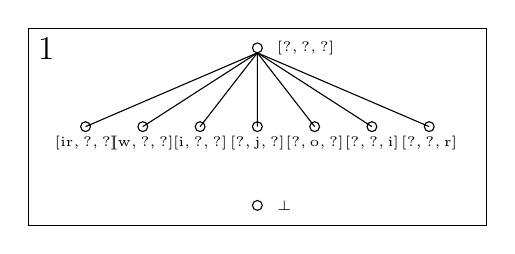
\begin{tikzpicture}
\def\delt{0.06*\textwidth};
\draw (-0.24*\textwidth,-1.25) rectangle (0.24*\textwidth,1.25);
\draw (-0.24*\textwidth,1.25) node[anchor=north west]{\large 1};
\draw (0,1) circle (0.0625);
\draw (0.125,1) node[anchor=west] {\tiny \sout{$\left[?,?,?\right]$}};
\draw (-3*\delt,0) circle (0.0625) node[anchor=north] {\tiny $\left[\mbox{ir},?,?\right]$} -- (0,0.9375);
\draw (-2*\delt,0) circle (0.0625) node[anchor=north] {\tiny $\left[\mbox{w},?,?\right]$} -- (0,0.9375);
\draw (-1*\delt,0) circle (0.0625) node[anchor=north] {\tiny $\left[\mbox{i},?,?\right]$} -- (0,0.9375);
\draw (0,0) circle (0.0625) node[anchor=north] {\tiny $\left[?,\mbox{j},?\right]$} -- (0,0.9375);
\draw (1*\delt,0) circle (0.0625) node[anchor=north] {\tiny $\left[?,\mbox{o},?\right]$} -- (0,0.9375);
\draw (2*\delt,0) circle (0.0625) node[anchor=north] {\tiny $\left[?,?,\mbox{i}\right]$} -- (0,0.9375);
\draw (3*\delt,0) circle (0.0625) node[anchor=north] {\tiny $\left[?,?,\mbox{r}\right]$} -- (0,0.9375);
\draw (0,-1) circle (0.0625);
\draw (0.125,-1) node[anchor=west] {\tiny $\perp$};
\end{tikzpicture}
}
\subfigure{
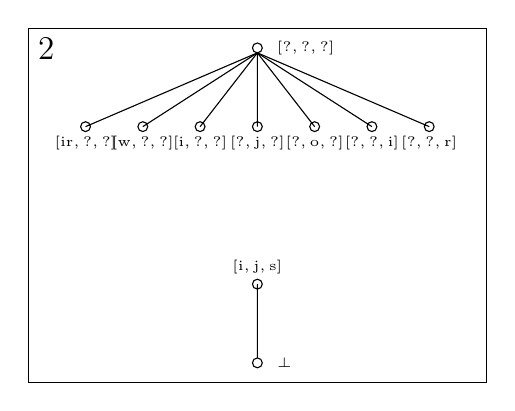
\begin{tikzpicture}
\def\delt{0.06*\textwidth};
\draw (-0.24*\textwidth,-2.25) rectangle (0.24*\textwidth,2.25);
\draw (-0.24*\textwidth,2.25) node[anchor=north west]{\large 2};
\draw (0,2) circle (0.0625);
\draw (0.125,2) node[anchor=west] {\tiny \sout{$\left[?,?,?\right]$}};
\draw (-3*\delt,1) circle (0.0625) node[anchor=north] {\tiny \sout{$\left[\mbox{ir},?,?\right]$}} -- (0,1.9375);
\draw (-2*\delt,1) circle (0.0625) node[anchor=north] {\tiny \sout{$\left[\mbox{w},?,?\right]$}} -- (0,1.9375);
\draw (-1*\delt,1) circle (0.0625) node[anchor=north] {\tiny $\left[\mbox{i},?,?\right]$} -- (0,1.9375);
\draw (0,1) circle (0.0625) node[anchor=north] {\tiny $\left[?,\mbox{j},?\right]$} -- (0,1.9375);
\draw (1*\delt,1) circle (0.0625) node[anchor=north] {\tiny \sout{$\left[?,\mbox{o},?\right]$}} -- (0,1.9375);
\draw (2*\delt,1) circle (0.0625) node[anchor=north] {\tiny $\left[?,?,\mbox{i}\right]$} -- (0,1.9375);
\draw (3*\delt,1) circle (0.0625) node[anchor=north] {\tiny $\left[?,?,\mbox{r}\right]$} -- (0,1.9375);
\draw (0,-1) circle (0.0625) node[anchor=south] {\tiny $\left[\mbox{i},\mbox{j},\mbox{s}\right]$} -- (0,-1.9375);
\draw (0,-2) circle (0.0625);
\draw (0.125,-2) node[anchor=west] {\tiny \sout{$\perp$}};
\end{tikzpicture}
}
\subfigure{
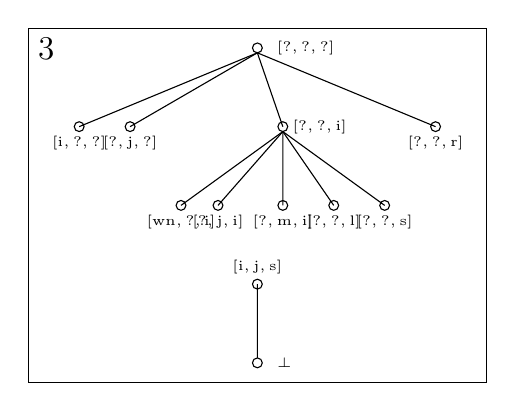
\begin{tikzpicture}
\def\delt{0.05333*\textwidth};
\draw (-0.24*\textwidth,-2.25) rectangle (0.24*\textwidth,2.25);
\draw (-0.24*\textwidth,2.25) node[anchor=north west]{\large 3};
\draw (0,2) circle (0.0625);
\draw (0.125,2) node[anchor=west] {\tiny \sout{$\left[?,?,?\right]$}};
\draw (-3.5*\delt,1) circle (0.0625) node[anchor=north] {\tiny $\left[\mbox{i},?,?\right]$} -- (0,1.9375);
\draw (-2.5*\delt,1) circle (0.0625) node[anchor=north] {\tiny $\left[?,\mbox{j},?\right]$} -- (0,1.9375);
\draw (0.5*\delt,1) circle (0.0625) node[anchor=west] {\tiny \sout{$\left[?,?,\mbox{i}\right]$}} -- (0,1.9375);
\draw (-1.5*\delt,0) circle (0.0625) node[anchor=north] {\tiny $\left[\mbox{wn},?,\mbox{i}\right]$} -- (0.5*\delt,0.9375);
\draw (-0.5,0) circle (0.0625) node[anchor=north] {\tiny \sout{$\left[?,\mbox{j},\mbox{i}\right]$}} -- (0.5*\delt,0.9375);
\draw (0.5*\delt,0) circle (0.0625) node[anchor=north] {\tiny \sout{$\left[?,\mbox{m},\mbox{i}\right]$}} -- (0.5*\delt,0.9375);
\draw (1.5*\delt,0) circle (0.0625) node[anchor=north] {\tiny \sout{$\left[?,?,\mbox{l}\right]$}} -- (0.5*\delt,0.9375);
\draw (2.5*\delt,0) circle (0.0625) node[anchor=north] {\tiny \sout{$\left[?,?,\mbox{s}\right]$}} -- (0.5*\delt,0.9375);
\draw (3.5*\delt,1) circle (0.0625) node[anchor=north] {\tiny $\left[?,?,\mbox{r}\right]$} -- (0,1.9375);
\draw (0,-1) circle (0.0625) node[anchor=south] {\tiny $\left[\mbox{i},\mbox{j},\mbox{s}\right]$} -- (0,-1.9375);
\draw (0,-2) circle (0.0625);
\draw (0.125,-2) node[anchor=west] {\tiny \sout{$\perp$}};
\end{tikzpicture}
}
\subfigure{
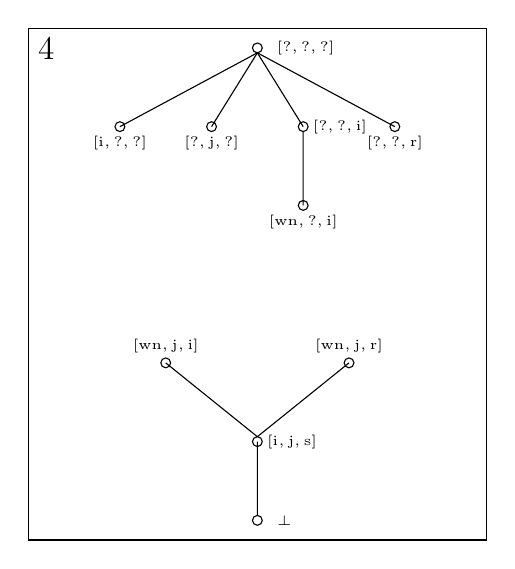
\begin{tikzpicture}
\def\delt{0.096*\textwidth};
\draw (-0.24*\textwidth,-3.25) rectangle (0.24*\textwidth,3.25);
\draw (-0.24*\textwidth,3.25) node[anchor=north west]{\large 4};
\draw (0,3) circle (0.0625);
\draw (0.125,3) node[anchor=west] {\tiny \sout{$\left[?,?,?\right]$}};
\draw (-1.5*\delt,2) circle (0.0625) node[anchor=north] {\tiny \sout{$\left[\mbox{i},?,?\right]$}} -- (0,2.9375);
\draw (-0.5*\delt,2) circle (0.0625) node[anchor=north] {\tiny $\left[?,\mbox{j},?\right]$} -- (0,2.9375);
\draw (0.5*\delt,2) circle (0.0625) node[anchor=west] {\tiny \sout{$\left[?,?,\mbox{i}\right]$}} -- (0,2.9375);
\draw (0.5*\delt,1) circle (0.0625) node[anchor=north] {\tiny $\left[\mbox{wn},?,\mbox{i}\right]$} -- (0.5*\delt,1.9375);
\draw (1.5*\delt,2) circle (0.0625) node[anchor=north] {\tiny $\left[?,?,\mbox{r}\right]$} -- (0,2.9375);
\draw (-1*\delt,-1) circle (0.0625) node[anchor=south] {\tiny $\left[\mbox{wn},\mbox{j},\mbox{i}\right]$} -- (0,-1.9375);
\draw (1*\delt,-1) circle (0.0625) node[anchor=south] {\tiny $\left[\mbox{wn},\mbox{j},\mbox{r}\right]$} -- (0,-1.9375);
\draw (0,-2) circle (0.0625) node[anchor=west] {\tiny \sout{$\left[\mbox{i},\mbox{j},\mbox{s}\right]$}} -- (0,-2.9375);
\draw (0,-3) circle (0.0625);
\draw (0.125,-3) node[anchor=west] {\tiny \sout{$\perp$}};
\end{tikzpicture}
}
\subfigure{
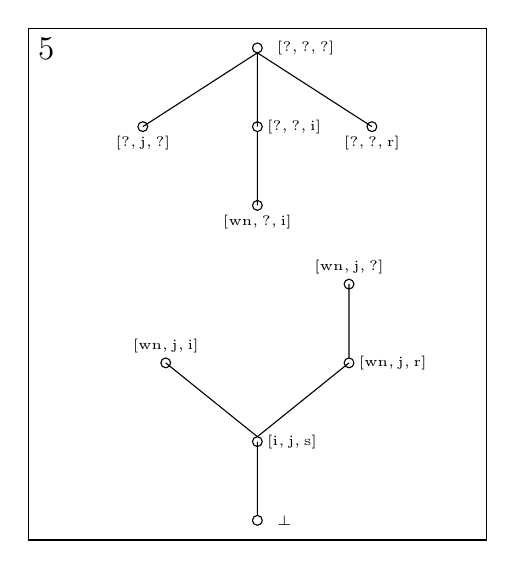
\begin{tikzpicture}
\def\dels{0.12*\textwidth};
\def\delt{0.096*\textwidth};
\draw (-0.24*\textwidth,-3.25) rectangle (0.24*\textwidth,3.25);
\draw (-0.24*\textwidth,3.25) node[anchor=north west]{\large 5};
\draw (0,3) circle (0.0625);
\draw (0.125,3) node[anchor=west] {\tiny \sout{$\left[?,?,?\right]$}};
\draw (-1*\dels,2) circle (0.0625) node[anchor=north] {\tiny $\left[?,\mbox{j},?\right]$} -- (0,2.9375);
\draw (0,2) circle (0.0625) node[anchor=west] {\tiny \sout{$\left[?,?,\mbox{i}\right]$}} -- (0,2.9375);
\draw (0,1) circle (0.0625) node[anchor=north] {\tiny $\left[\mbox{wn},?,\mbox{i}\right]$} -- (0,1.9375);
\draw (1*\dels,2) circle (0.0625) node[anchor=north] {\tiny \sout{$\left[?,?,\mbox{r}\right]$}} -- (0,2.9375);
\draw (1*\delt,0) circle (0.0625) node[anchor=south] {\tiny \sout{$\left[\mbox{wn},\mbox{j},\mbox{?}\right]$}} -- (\delt,-0.9375);
\draw (-1*\delt,-1) circle (0.0625) node[anchor=south] {\tiny $\left[\mbox{wn},\mbox{j},\mbox{i}\right]$} -- (0,-1.9375);
\draw (1*\delt,-1) circle (0.0625) node[anchor=west] {\tiny \sout{$\left[\mbox{wn},\mbox{j},\mbox{r}\right]$}} -- (0,-1.9375);
\draw (0,-2) circle (0.0625) node[anchor=west] {\tiny \sout{$\left[\mbox{i},\mbox{j},\mbox{s}\right]$}} -- (0,-2.9375);
\draw (0,-3) circle (0.0625);
\draw (0.125,-3) node[anchor=west] {\tiny \sout{$\perp$}};
\end{tikzpicture}
}
\subfigure{
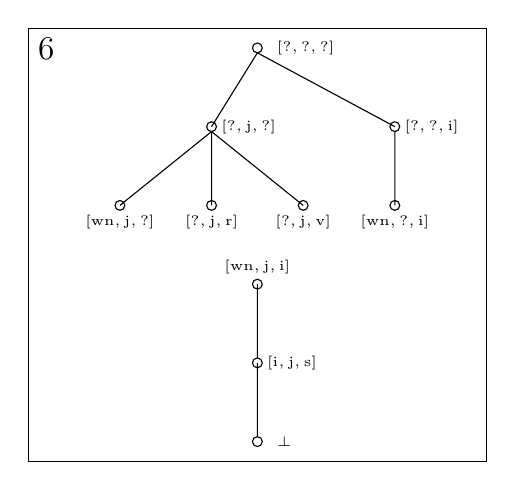
\begin{tikzpicture}
\def\delt{0.096*\textwidth};
\draw (-0.24*\textwidth,-2.25) rectangle (0.24*\textwidth,3.25);
\draw (-0.24*\textwidth,3.25) node[anchor=north west]{\large 6};
\draw (0,3) circle (0.0625);
\draw (0.125,3) node[anchor=west] {\tiny \sout{$\left[?,?,?\right]$}};
\draw (-0.5*\delt,2) circle (0.0625) node[anchor=west] {\tiny \sout{$\left[?,\mbox{j},?\right]$}} -- (0,2.9375);
\draw (-1.5*\delt,1) circle (0.0625) node[anchor=north] {\tiny $\left[\mbox{wn},\mbox{j},?\right]$} -- (-0.5*\delt,1.9375);
\draw (-0.5*\delt,1) circle (0.0625) node[anchor=north] {\tiny \sout{$\left[?,\mbox{j},\mbox{r}\right]$}} -- (-0.5*\delt,1.9375);
\draw (0.5*\delt,1) circle (0.0625) node[anchor=north] {\tiny \sout{$\left[?,\mbox{j},\mbox{v}\right]$}} -- (-0.5*\delt,1.9375);
\draw (1.5*\delt,2) circle (0.0625) node[anchor=west] {\tiny \sout{$\left[?,?,\mbox{i}\right]$}} -- (0,2.9375);
\draw (1.5*\delt,1) circle (0.0625) node[anchor=north] {\tiny $\left[\mbox{wn},?,\mbox{i}\right]$} -- (1.5*\delt,1.9375);
\draw (0,0) circle (0.0625) node[anchor=south] {\tiny $\left[\mbox{wn},\mbox{j},\mbox{i}\right]$} -- (0,-0.9375);
\draw (0,-1) circle (0.0625) node[anchor=west] {\tiny \sout{$\left[\mbox{i},\mbox{j},\mbox{s}\right]$}} -- (0,-1.9375);
\draw (0,-2) circle (0.0625);
\draw (0.125,-2) node[anchor=west] {\tiny \sout{$\perp$}};
\end{tikzpicture}
}
\subfigure{
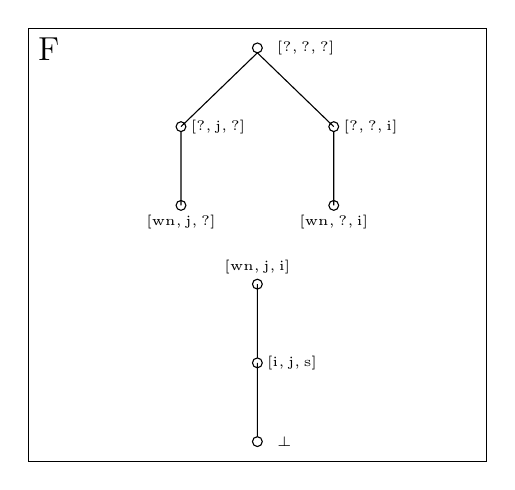
\begin{tikzpicture}
\def\delt{0.16*\textwidth};
\draw (-0.24*\textwidth,-2.25) rectangle (0.24*\textwidth,3.25);
\draw (-0.24*\textwidth,3.25) node[anchor=north west]{\large F};
\draw (0,3) circle (0.0625);
\draw (0.125,3) node[anchor=west] {\tiny \sout{$\left[?,?,?\right]$}};
\draw (-0.5*\delt,2) circle (0.0625) node[anchor=west] {\tiny \sout{$\left[?,\mbox{j},?\right]$}} -- (0,2.9375);
\draw (-0.5*\delt,1) circle (0.0625) node[anchor=north] {\tiny $\left[\mbox{wn},\mbox{j},?\right]$} -- (-0.5*\delt,1.9375);
\draw (0.5*\delt,2) circle (0.0625) node[anchor=west] {\tiny \sout{$\left[?,?,\mbox{i}\right]$}} -- (0,2.9375);
\draw (0.5*\delt,1) circle (0.0625) node[anchor=north] {\tiny $\left[\mbox{wn},?,\mbox{i}\right]$} -- (0.5*\delt,1.9375);
\draw (0,0) circle (0.0625) node[anchor=south] {\tiny $\left[\mbox{wn},\mbox{j},\mbox{i}\right]$} -- (0,-0.9375);
\draw (0,-1) circle (0.0625) node[anchor=west] {\tiny \sout{$\left[\mbox{i},\mbox{j},\mbox{s}\right]$}} -- (0,-1.9375);
\draw (0,-2) circle (0.0625);
\draw (0.125,-2) node[anchor=west] {\tiny \sout{$\perp$}};
\end{tikzpicture}
}
\caption{Verloop van Version Spaces op de testdata.}
\label{fig:versionSpacesExampleFull}
\end{figure}
\paragraph{Het beslissingsalgoritme}
Naast het leren van een concept moeten Version Spaces uiteindelijk ook kunnen beslissen of een gegeven situatie wel degelijk deel uitmaakt van het concept. Indien de gebruiker vraagt of een bepaalde situatie tot het concept behoort, zal het beslissingalgoritme testen of iedere hypothese (zowel in $G$ als in $S$) deze situatie juist beslist. Nochtans hoeven we enkel de hypotheses van $S$ te testen om te besluiten dat een situatie wel degelijk positief is, $G$ bevat immers alleen maar generalisaties van $S$ en zal dus bijgevolg ook altijd juist testen. Omgekeerd hoeven we alleen de hypotheses van $G$ te testen om te besluiten dat iedere hypothese de situatie verwerpt. Het probleem is uiteraard dat een situatie wel eens door verschillende hypotheses anders beoordeeld kan worden. In dat geval wordt meestal de ratio tussen positieve en negatieve beoordelingen berekend en wordt afhankelijk hiervan een positief of negatief resultaat teruggegeven, meestal met vermelding van de probabiliteit. Indien er echter evenveel positieve als negatieve beoordelingen zijn wordt er meestal geen conclusie getrokken. Een compacte implementatie hiervoor wordt beschreven in \algref{alg:versionSpacesConclusion}.
\begin{algorithm}[htb]                      % enter the algorithm environment
\caption{Conclusie trekken uit een Version-space}          % give the algorithm a caption
\label{alg:versionSpacesConclusion}                           % and a label for \ref{} commands later in the document
\begin{algorithmic}[1]                    % enter the algorithmic environment
\STATE$n^+\leftarrow0$
\STATE$n^-\leftarrow0$
\FORALL{$h\in S\cup G$}
\IF{$\hypothesiscovers{h,d}$}
\STATE$n^+\leftarrow n^++1$
\ELSE
\STATE$n^-\leftarrow n^-+1$
\ENDIF
\ENDFOR
\IF{$n^-=0$}
\RETURN $\true$
\ELSIF{$n^+=0$}
\RETURN $\false$
\ELSIF{$n^+>n^-$}
\RETURN ``$\true$ with a probability of $n^+/(n^++n^-)$''
\ELSIF{$n^+<n^-$}
\RETURN ``$\false$ with a probability of $n^-/(n^++n^-)$''
\ELSE[$n^+=n^-$]
\RETURN ``no conclusion''
\ENDIF
\end{algorithmic}
\end{algorithm}
\subsection{De relevantie van de hypothesetaal}
\label{sss:relevanceHypothesisLanguage}
De hierboven gestelde hypothesetaal slaagt er niet in om alle mogelijke concepten te leren (omdat er bijvoorbeeld enkel generalisaties zijn die later tegengesproken worden door een ander voorbeeld). Kunnen we met een expressievere taal eventueel betere concepten aanleren? Stel dat we een nieuwe taal defini\"eren die opnieuw werkt door middel van symbolen. Hierbij defini\"eren we elementen van de vorm $<\mbox{parameter}>=<\mbox{waarde}>$. Verder laten we conjuncties (die ook al toegelaten waren), disjuncties en negaties toe. Deze taal kan met andere woorden iedere deelverzameling van mogelijke staten bevatten (elke staat valt te beschrijven door een conjunctie van al haar parameters, met een disjunctie kunnen we deze combineren). Het probleem is dat we weer tot dezelfde resultaten komen als onze na\"ieve implementatie in het begin (zie \ref{sss:versionSpacesNaif}). En we dus met andere woorden niets kunnen leren. We geven enkel waar indien we de situatie al positieve gedaante zagen in de testdata, en negatief indien de situatie als negatief voorbeeld in de test-data stond. We kunnen dus stellen dat we nood hebben aan een \termen{Inductieve BIAS}, dit is een aanname dat het concept kan geleerd worden door een bepaalde set regels voor een hypothesetaal (Zo is de hypothesetaal hierboven te beschrijven als een conjunctie van eigenschappen).
\paragraph{}Hoe weten we echter of onze hypothesetaal zal volstaan? Dit is uiteraard niet op voorhand te bepalen. In de loop der tijd zijn er echter verschillende hypothesetalen ontstaan. We kunnen een orde specifi\"eren in de talen naar representatievermogen. Veel praktische algoritmen hebben dan ook een set van dergelijke talen. Indien de gebruiker niet tevreden is met de resultaten van een beperkte hypothesetaal, verandert het algoritme de taal naar een hypothesetaal met een breder representatievermogen. Dit vermijdt de keuze van een taal, bovendien zal de minst representatieve taal het meest algemene concept genereren, waardoor het concept waarschijnlijk dan ook het best gedefinieerd zal zijn.
